\begin{frame}
	\myheading{Module 5.2: Learning Parameters : Gradient Descent}
\end{frame}

\begin{frame}
	\fontsize{16pt}{7.2}\selectfont
	\textit{Now let's see if there is a more efficient and principled way of doing this}
\end{frame}

%\section{Optimization methods}
%\subsection{Gradient Descent}
%\subsection{Goal}
\begin{frame}
	\begin{block}{Goal}
		Find a better way of traversing the error surface so that we can reach the minimum value quickly without resorting to brute force search! 
	\end{block}
\end{frame}


\begin{frame}
	\begin{overlayarea}{\textwidth}{\textheight}
		\begin{tikzpicture}
\begin{axis}[axis lines=left, ticks=none,xmax=0.5,ymax=0.5,x label style={at={(axis description cs:0.5,0)},anchor=north},
xlabel={$\theta$}, ylabel={error}]
\addplot[thick,black, no markers, samples=200, domain=-5:0] {-x*exp(x)};
\only<2->{\draw[dashed] (axis cs:-1.88,0.31) -- (axis cs:-0.0,0.31)} ;
\only<2->{\draw[dashed] (axis cs:-2.68,0.21) -- (axis cs:-0.0,0.21)} ;

\end{axis}
\end{tikzpicture}

	\end{overlayarea}
	
\end{frame}

%\subsection{Taylor series}
\begin{frame}
	\begin{overlayarea}{\textwidth}{\textheight}
		For ease of notation, let $\Delta\theta = u$, then from Taylor series, we have,
		
		\begin{align*}
			\only<2->{\mathscr{L}(\theta + \eta u) & =  \mathscr{L}(\theta)+ \eta*u^T \nabla\mathscr{L}(\theta) + \frac{\eta^2}{2!}*u^T \nabla^2\mathscr{L}(\theta)u + \frac{\eta^3}{3!}*... + \frac{\eta^4}{4!}*...} \\
			\only<3->{                             & = \mathscr{L}(\theta)+ \eta*u^T \nabla\mathscr{L}(\theta) \text{  } [\textit{$\eta$ is typically small, so $\eta^2, \eta^3,...\rightarrow 0$}]}                  
		\end{align*}
		
		\only<4->{Note that the move ($\eta u$) would be favorable only if,}
		\begin{align*}
			\only<4->{ & \mathscr{L}(\theta + \eta u) - \mathscr{L}(\theta) < 0 \textit{ }[\textit{i.e., if the new loss is less than the previous loss}]} \\
			\only<5->{\intertext {This implies,}}
			\only<5->{ & u^T \nabla\mathscr{L}(\theta) < 0}                                                                                      
		\end{align*}
	\end{overlayarea}
\end{frame}

\begin{frame}
	
	\begin{overlayarea}{\textwidth}{\textheight}
		Okay, so we have,
		\begin{align*}
			u^T \nabla\mathscr{L}(\theta) < 0 
		\end{align*}
		
		\only<1->{But, what is the range of $u^T \nabla\mathscr{L}(\theta)$ ?} \only<2->{Let's see....}\\
		
		\only<3->{Let $\beta$ be the angle between $u^T$ and $\nabla\mathscr{L}(\theta)$, then we know that,} 
		\only<4->{
			\begin{align*}
				\onslide<4->{-1 & \leq cos(\beta) = \frac{u^T \nabla\mathscr{L}(\theta)}{||u||*||\nabla\mathscr{L}(\theta)||} \leq 1} 
				%\only<5->{\intertext{Let's assume $u$ and $\mathscr{L}'(\theta)$ are unit vectors}}
				\onslide<5->{\intertext{Multiply throughout by $k = ||u||*||\nabla\mathscr{L}(\theta)||$ }}
				\onslide<5->{-k & \leq k*cos(\beta) = u^T \nabla\mathscr{L}(\theta) \leq k }                                          
				\onslide<6->{\intertext{Thus, $\mathscr{L}(\theta + \eta u) - \mathscr{L}(\theta) = u^T \nabla\mathscr{L}(\theta) = k*cos(\beta)$ will be most negative when $cos(\beta) =-1$ \textit{i.e.}, when $\beta$ is $180\degree$}}
			\end{align*}
		}
		
	\end{overlayarea}
\end{frame}

%\subsection{The update rule}
\begin{frame}
	\begin{overlayarea}{\textwidth}{\textheight}
		
		\begin{block}{Gradient Descent Rule}
			\begin{itemize}\justifying
				\item<1-> The direction $u$ that we intend to move in should be at $180\degree$ w.r.t. the gradient
				\item<2-> In other words, move in a direction opposite to the gradient
			\end{itemize}
		\end{block}
		
		\only<3->{
			\begin{block}{Parameter Update Equations}
				\vspace{-0.1in}
				\begin{align*}
					w_{t+1}             & = w_{t} - \eta \nabla w_{t}                                                 \\
					b_{t+1}             & = b_{t} - \eta \nabla b_{t}                                                 \\
					where, \nabla w_{t} & = \frac{\partial\mathscr{L}(w,b)}{\partial w}_{\textit{at $w=w_t, b=b_t$}}, 
					\nabla b_t = \frac{\partial\mathscr{L}(w,b)}{\partial b}_{\textit{at $w=w_t, b=b_t$}}
				\end{align*}
			\end{block}
		}
		
		\only<4-> {So we now have a more principled way of moving in the $w$-$b$ plane than our ``guess work'' algorithm}
		
		
	\end{overlayarea}
\end{frame}

\begin{frame}
	\begin{overlayarea}{\textwidth}{\textheight}
		
		\begin{itemize}\justifying
			    
			\item <1-> Let's create an algorithm from this rule ... 
			      
			      \only<2-> {
			      	\begin{algorithm}[H]
			      		\SetAlgoLined
			      		$t \leftarrow 0$\; 
			      		$max\_iterations\leftarrow 1000$\;
			      		\While{$t < max\_iterations$}{
			      			$w_{t+1} \leftarrow w_{t} - \eta \nabla w_{t}$\;
			      			$b_{t+1} \leftarrow b_{t} - \eta \nabla b_{t}$\;
			      		}
			      		\caption{gradient\_descent()}
			      	\end{algorithm}
			      }
			      
			\item <2-> To see this algorithm in practice let us first derive $\nabla w$ and $\nabla b$ for our toy neural network
			      
		\end{itemize}
		
	\end{overlayarea}
	
\end{frame}

\begin{frame}
	\begin{columns}
		
		\column{0.5\textwidth}
		\begin{overlayarea}{\textwidth}{\textheight}
			\tikzstyle{neuron}=[circle,draw=blue!50,fill=blue!20,thick,minimum size=10mm]
\tikzstyle{input}=[circle,draw=black!50,fill=black!20,thick,minimum size=6mm]
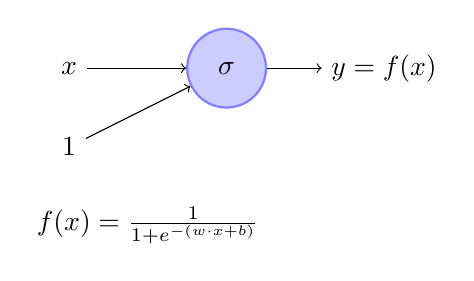
\begin{tikzpicture}
\node [neuron] (neuron0) at (1,6)  {$\sigma$} ;
\node (input1) at (-1,6)  {$x$};
\node (input0) at (-1,5)  {$1$};
\node (output0) at (3,6)  {$y = f(x)$};
\node (formula) at (0,4) {$f(x)= \frac{1}{1+e^{-(w\cdot x + b)}}$};
\draw [->] (input0) -- (neuron0);
\draw [->] (input1) -- (neuron0);
\draw [->] (neuron0) -- (output0);
\end{tikzpicture}

			\vspace{-0.2in}
			\begin{figure}[!htp]
				\begin{center}
					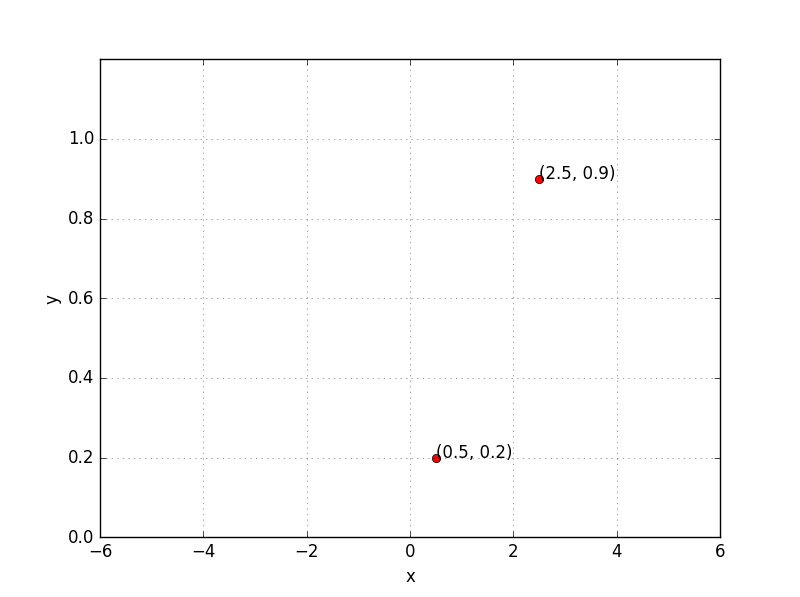
\includegraphics[scale=0.3]{images/module2/2sample_points.png}
				\end{center}
			\end{figure}
			
		\end{overlayarea}
		
		\column{0.5\textwidth}<2->
		\begin{overlayarea}{\textwidth}{\textheight}
			\begin{align*}
				\onslide<2->{\intertext{Let's assume there is only 1 point to fit $(x, y)$}}
				\onslide<3->{\mathscr{L}(w,b)                                       & = \frac{1}{2} * (f(x) - y)^2                               \\} 
				\onslide<4->{\nabla w = \frac{\partial\mathscr{L}(w,b)}{\partial w} & = \frac{\partial}{\partial w} [\frac{1}{2} * (f(x) - y)^2] \\} 
			\end{align*}
			
		\end{overlayarea}
	\end{columns}
\end{frame}

\begin{frame}
	\begin{columns}
		\begin{column}{0.46\textwidth}
			\begin{overlayarea}{\textwidth}{\textheight}
				\begin{align*}
					\onslide<1->\nabla w & = \frac{\partial}{\partial w} [\frac{1}{2} * (f(x) - y)^2]                      \\
					\onslide<2->{        & = \frac{1}{2} * [2*(f(x) - y) * \frac{\partial}{\partial w}(f(x) - y)]          \\}
					\onslide<3->{        & = (f(x) - y) * \frac{\partial}{\partial w}(f(x))                                \\}
					\onslide<4->{        & = (f(x) - y) * \frac{\partial}{\partial w}\Big(\frac{1}{1 + e^{-(wx + b)}}\Big) \\}
					\onslide<10->{       & = \color{red}{(f(x) - y) * f(x)*(1- f(x)) *x}}                                  
				\end{align*}
			\end{overlayarea}
		\end{column}
		
		\vrule{}
		
		\begin{column}{0.54\textwidth}
			\begin{overlayarea}{\textwidth}{\textheight}
				
				\begin{align*}
					\onslide<5->{ & \frac{\partial}{\partial w}\Big(\frac{1}{1 + e^{-(wx + b)}}\Big)                         \\}
					\onslide<6->{ & =\frac{-1}{(1 + e^{-(wx + b)})^2}\frac{\partial}{\partial w}(e^{-(wx + b)}))             \\}
					\onslide<7->{ & =\frac{-1}{(1 + e^{-(wx + b)})^2}*(e^{-(wx + b)})\frac{\partial}{\partial w}(-(wx + b))) \\}
					\onslide<8->{ & =\frac{-1}{(1 + e^{-(wx + b)})}*\frac{e^{-(wx + b)}}{(1 + e^{-(wx + b)})} *(-x)          \\}
					\onslide<8->{ & =\frac{1}{(1 + e^{-(wx + b)})}*\frac{e^{-(wx + b)}}{(1 + e^{-(wx + b)})} *(x)            \\}
					\onslide<9->{ & =f(x)*(1- f(x))*x}                                                                       
				\end{align*}
			\end{overlayarea}
		\end{column}
		
	\end{columns}
	
\end{frame}


\begin{frame}
	\begin{columns}
		
		\column{0.45\textwidth}
		\begin{overlayarea}{\textwidth}{\textheight}
			\tikzstyle{neuron}=[circle,draw=blue!50,fill=blue!20,thick,minimum size=10mm]
\tikzstyle{input}=[circle,draw=black!50,fill=black!20,thick,minimum size=6mm]
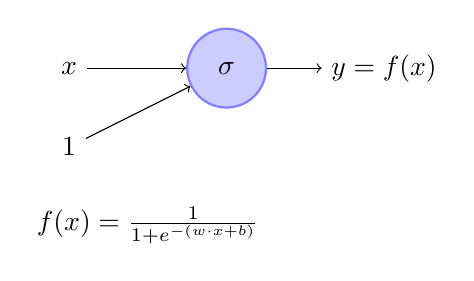
\begin{tikzpicture}
\node [neuron] (neuron0) at (1,6)  {$\sigma$} ;
\node (input1) at (-1,6)  {$x$};
\node (input0) at (-1,5)  {$1$};
\node (output0) at (3,6)  {$y = f(x)$};
\node (formula) at (0,4) {$f(x)= \frac{1}{1+e^{-(w\cdot x + b)}}$};
\draw [->] (input0) -- (neuron0);
\draw [->] (input1) -- (neuron0);
\draw [->] (neuron0) -- (output0);
\end{tikzpicture}

			\vspace{-0.2in}
			\begin{figure}[!htp]
				\begin{center}
					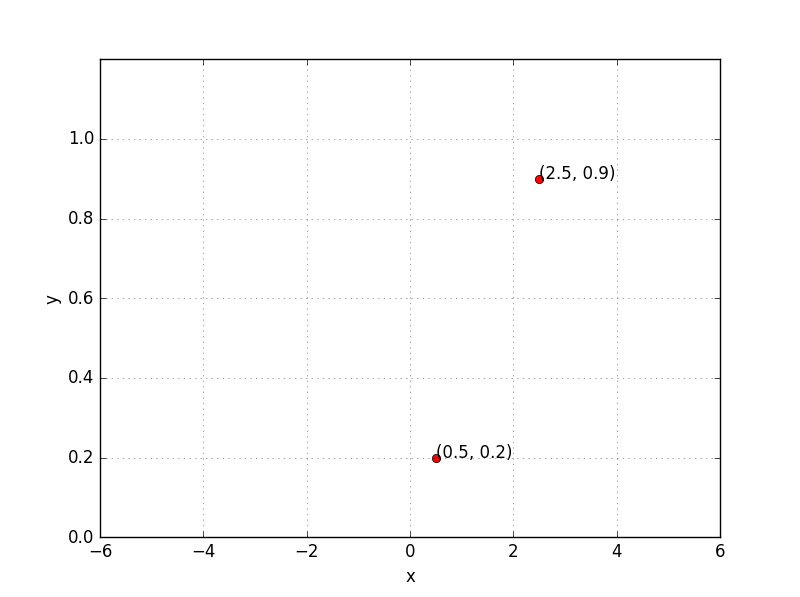
\includegraphics[scale=0.3]{images/module2/2sample_points.png}
				\end{center}
			\end{figure}
			
		\end{overlayarea}
		
		\column{0.55\textwidth}<1->
		\begin{overlayarea}{\textwidth}{\textheight}
			\begin{align*}
				\onslide<1->{\intertext{So if there is only 1 point $(x, y)$, we have, }}
				%\only<1->{\mathscr{L}(w,b) &= \frac{1}{2} * (f(x) - y)^2 \\} 
				%    \only<1->{\nabla w &= \frac{\partial\mathscr{L}(w,b)}{\partial w} &= \frac{\partial}{\partial w} [\frac{1}{2} * (f(x) - y)^2] \\} 
				\onslide<2->{\nabla w & = (f(x) - y) * f(x)*(1- f(x)) *x}                          
				\onslide<3->{\intertext{For two points,}}
				\onslide<4->{\nabla w & = \sum_{i=1}^{2} (f(x_i) - y_i) * f(x_i)*(1- f(x_i)) *x_i} \\
				%\only<5->{\intertext{Similarly}}
				\onslide<5->{\nabla b & = \sum_{i=1}^{2} (f(x_i) - y_i) * f(x_i)*(1- f(x_i))}      
			\end{align*}
			
		\end{overlayarea}
	\end{columns}
\end{frame}


% \begin{frame}
% 	\begin{columns}
		
% 		\column{0.5\textwidth}
% 		\begin{overlayarea}{\textwidth}{\textheight}
% 			\vspace{-0.15in}
% 			\begin{figure}
% 				\includegraphics<1>[clip,trim=0 650 0 0,scale=0.3]{images/module2/pseudo_code_sgd_crop.png}
% 				\includegraphics<2>[clip,trim=0 580 0 0,scale=0.3]{images/module2/pseudo_code_sgd_crop.png}
% 				\includegraphics<3-4>[clip,trim=0 415 0 0,scale=0.3]{images/module2/pseudo_code_sgd_crop.png}
% 				\includegraphics<5>[clip,trim=0 325 0 0,scale=0.3]{images/module2/pseudo_code_sgd_crop.png}
% 				\includegraphics<6>[clip,trim=0 235 0 0,scale=0.3]{images/module2/pseudo_code_sgd_crop.png}
% 				\includegraphics<7>[scale=0.3]{images/module2/pseudo_code_sgd_crop.png}
% 			\end{figure}
% 		\end{overlayarea}
		
% 		\column{0.5\textwidth}
% 		\begin{overlayarea}{\textwidth}{\textheight}
			
			
% 			\begin{figure}
% 				% \includegraphics<4->[scale=0.5]{images/module2/error_surface1.png}
% 				\includegraphics<4->[scale=0.5]{images/module2/sgd0/sgd_error0.png}
% 			\end{figure}
			
% 			%<4>Why are the changes in  w \& b so small ?
% 			%<5>Why do we see larger changes in  w \& b now ?
% 			%<6>And again the changes in  w \& b become small. Why ?
% 		\end{overlayarea}
		
% 	\end{columns}
% \end{frame}


\begin{frame}
	
	\begin{columns}
		\column{0.5\textwidth}
		\begin{overlayarea}{\textwidth}{\textheight}
			\vspace{-0.15in}
			\begin{figure}
				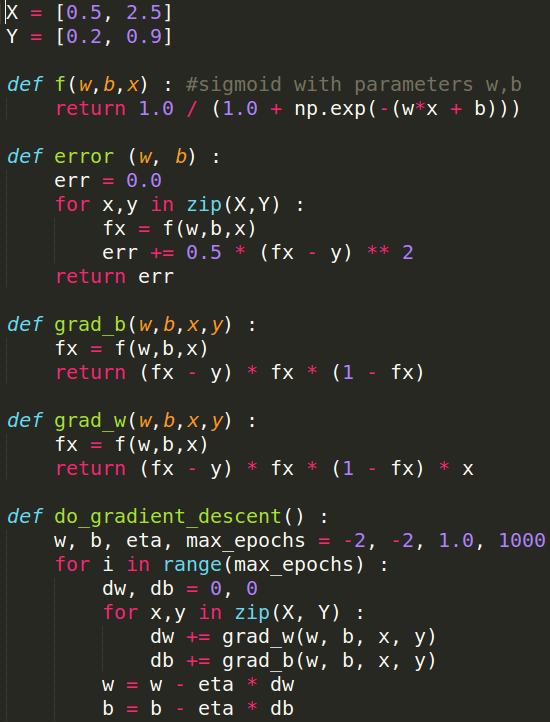
\includegraphics[scale=0.3]{images/module2/pseudo_code_sgd_crop.png}
			\end{figure}
		\end{overlayarea}
		
		\column{0.5\textwidth}
		\begin{overlayarea}{\textwidth}{\textheight}
			\vspace{-0.15in}
			
			%\animategraphics[scale=0.5]{12}{images/module2/sgd0/sgd_error}{0}{99}
			
			\begin{figure}
				\foreach \n in {0,...,99} {%
					\includegraphics<\n>[scale=0.5]{images/module2/sgd0/sgd_error\n.png}
				}
			\end{figure}
		\end{overlayarea}
		
	\end{columns}
\end{frame}

\begin{frame}
	
	\begin{columns}
		
		\column{0.5\textwidth}
		\begin{tikzpicture} 
  \tkzInit[xmin=-1,xmax=4.5,ymax=6]
  \tkzClip[space=1]
    \tkzAxeXY
    \tkzFct[domain=.1:5,samples=200,id=ln,line width=0.5pt,color=red]{x**2 + 1} 
%    \tkzDrawTangentLine[kl=1,kr=5](1)
	\only<2->{\draw[domain=-1:2.2,smooth,variable=\x,red]  plot ({\x}, {\x*\x + 1}); }
    \tkzText[draw=red,fill = red!20](2.75, 6){$f(x)=x^2+1$}
    \only<3->{\derivative{1}{2}{$\Delta x_1$}{$\Delta y_1$}{above}}
    \only<3->{\draw[domain=-1:2.2,smooth,variable=\x,red]  plot ({\x}, {\x*\x + 1}); }
    \only<4->{\derivative{0}{1}{$\Delta x_2$}{$\Delta y_2$}{below}}   
  	
\end{tikzpicture} 

		\column{0.5\textwidth}
		\begin{overlayarea}{\textwidth}{\textheight}
			\begin{itemize}\justifying
				\item<2-> When the curve is steep the gradient ($\frac{\Delta y_1}{\Delta x_1}$) is large
				\item<3-> When the curve is gentle the gradient ($\frac{\Delta y_2}{\Delta x_2}$) is small
				\item<4-> Recall that our weight updates are proportional to the gradient $w = w - \eta \nabla w$
				\item<5-> Hence in the areas where the curve is gentle the updates are small whereas in the areas where the curve is steep the updates are large
			\end{itemize}
			
		\end{overlayarea}
	\end{columns}
	    
\end{frame}

\begin{frame}
	\fontsize{16pt}{7.2}\selectfont
	\begin{itemize}\justifying
		\item \textit{Let's see what happens when we start from a different point}
	\end{itemize}
\end{frame}

\begin{frame}
	
	\begin{columns}
		\column{0.5\textwidth}
		\begin{overlayarea}{\textwidth}{\textheight}
			\begin{itemize}\justifying
				\item<2-> Irrespective of where we start from once we hit a surface which has a gentle slope, the progress slows down
			\end{itemize}
		\end{overlayarea}
		
		\column{0.5\textwidth}
		\begin{overlayarea}{\textwidth}{\textheight}
			\vspace{-0.15in}
			
			%\animategraphics[scale=0.5]{12}{images/module2/sgd0/sgd_error}{0}{99}
			
			\begin{figure}
				\foreach \n in {0,...,129} {%
					\includegraphics<\n>[scale=0.5]{images/module2/sgd0.1/3d_path\n.png}
				}
			\end{figure}
		\end{overlayarea}
		
	\end{columns}
\end{frame}
